\chapter{Our Solution}
\label{kap:solution}
In~this chapter, we present our own solution to~the~electronic election system. We describe players in~the~final voting scheme we implement, the~voting scheme itself and the~format in~which the~vote is stored and read. Then, we bring some description of~existing security schemes and services we use in~our solution. We also discuss some other proposals of~the~voting scheme, which we modified or rejected. 

\section{Our Voting Scheme}
Our voting scheme is similar to~the~scheme that has been developed for~elections in~Estonia. This scheme is described in~chapter \ref{kap:existing}. Both schemes are based on~the~principle that voter's identity cannot be known to~any player besides that particular voter when their vote can~be decrypted or read. It means that computer that is responsible for~decrypting the~votes cannot obtain~any information about~any voter who casted their vote. 

We bear in~mind that we require the~voting process to~run in~an~Internet browser and that this technology has several limitations. The~reader can~read more about limitations of~the~technology used in~chapter \ref{kap:implementation}.
%We bear in~mind that we require voting application to~be run in~an~Internet browser.

\section{Players in~Our Voting Scheme}
We shortly describe each player in~our voting scheme and their purpose.
\begin{itemize}
\item \textbf{Voter $V$} authenticates to~$S$ using \emph{authentication authority $T$} and casts their vote using \emph{voting application $A$}. They also can~cast their vote in~paper form in~a~special-purpose room.
\item \textbf{Election commission $B$} are in~charge of~key generation during the~first phase. They hold secret key $SK$ generated for~\emph{machine for~vote counting $M$} and share corresponding public key $PK$. They also securely transfer encrypted data from \emph{server for~vote collection $S$} to~$M$. Data~can~be, then, decrypted using $SK$, provided to~$M$ by~$B$. In~the~end, they publish the~result of~the~elections. Last but not least, they are responsible for~paper votes casted in~a~special-purpose room designed for~the~elections.
\item \textbf{Database $D$} stores information about all the~candidates and identities of~all authorised voters. This information is then used by~$A$ and $S$ to~display list of~possible candidates and authorise \emph{voter $V$}. This database is physically stored on server $S$ and is accessible only to~$S$.
\item \textbf{Voting application $A$} provides user interface for~$V$ in~which they can~cast their vote. It also validates the~vote, converts it to~a~proper format and encrypts it using $PK$. Then it sends the~vote together with~the~voter's identity.
\item \textbf{Server for~vote collection $S$} receives encrypted vote and voter's identity and checks whether this identity corresponds to~any of~those stored in~\emph{database $D$}. If the~encrypted vote comes from~an~authorised voter, then it stores the~encrypted vote and the~voter's identity in~its internal database of~votes. This server also provides storage for~voting application $A$ and database $D$.
\item \textbf{Machine for~vote counting $M$} receives all the~votes (without identity of~any voter) stored in~$S$'s internal database and secret key $SK$. It, then, decrypts all the~received votes using $SK$, validates them and computes the~result of~the~elections, which is finally published. We point out that this machine is not connected to~any network prior or during the~elections. This machine is restricted to~be in~off-line mode until the~results of~the~elections are published and it is proved that the~election process has been correctly performed.
\item \textbf{Authentication authority $T$} is responsible for~authentication of~$V$ and provides $M$ with~$V$'s identity, which must \emph{1-to-1} correspond to~a~value in~$D$. For~purposes of~our voting scheme, we use \emph{Cosign}, which is a~service commonly used for~authentication of~students studying at our faculty. From~this point, we mean~\emph{Cosign} any time we talk about $T$. Similarly, we use term \emph{UK login} of~voter $V$ instead of~\emph{$V$'s identity}. More information about \emph{Cosign} is provided in~section \ref{sek:cryptography}  and chapter \ref{kap:implementation}.
\end{itemize}

\section{Phases of~Our Voting Scheme}
Our voting scheme is designed to~have three subsequent phases: \emph{initialisation phase}, \emph{voting phase} and \emph{counting phase}. The~basic purpose of~these stages is discussed in~chapter~\ref{kap:definition}. In~this section, we provide a~detailed description of~what is done during each of~these phases.

\subsection{Initialisation}
\begin{enumerate}
\item Database $D$ with~a~table of~candidates is created and stored on $S$. For~each candidate, the~table contains a~unique ID and name of~the~candidate.
\item A~table of~authorised voters is created in~$D$. For~each voter, this table contains their \emph{UK login} and a~boolean~variable set to~0. This variable indicates whether the~voter has already casted a~paper vote.
\item A~special \emph{UK login} is created for~the~election commission $B$. This login~is used when a~voter casts their paper vote.
\item Public key $PK$ and secret key $SK$ are generated. They are to~be used to~encrypt the~vote by~the~voting application $A$ and decrypt it by~the~machine for~vote counting $M$, respectively.
\item Using \emph{Shamir's Secret-Sharing Scheme}, the~key $SK$ is divided into~$n$ parts, where $n$ is the~number of~members of~$B$. The~key $SK$ can~be reconstructed from~any combination of~$k$ parts, where $k$ is the~smallest number of~members of~$B$ that have to~sign the~\emph{Protocol of~elections}. The~reader can~read more about the~scheme in~section \ref{sek:cryptography}.
\item Public key $PK$ is shared with~all the~voters by~inserting it into~$A$ as a~constant value for~the~whole elections.
\end{enumerate}

\subsection{Voting}
%This phase follows after initialisation was completed. \smallbreak
For~each voter $V$:
\begin{enumerate}
\item Voter $V$ opens a~specific Internet location in~their browser and logs in~using $Cosign$ in~order to~authenticate to~$S$.
\item If $V$ is successfully authenticated, voting application is launched in~their Internet browser. This application contains a~form in~which there are three options for~each candidate.
\item When $V$ submits the~form, it is then validated regarding the~rules of~the~elections. When form valid, vote in~the~format described in~section \ref{sek:format} is created and this vote is encrypted using \emph{S/MIME} protocol and $PK$. Finally, the~vote and voter's \emph{UK login} are sent to~$S$ via~an~\emph{HTTPS} connection.
\item When $S$ receives the~encrypted vote, it compares the~sender's \emph{UK login} with~logins in~the~table of~authorised voters stored in~$D$. If it matches exactly one record, then the~login~and the~encrypted vote are stored in~$S$'s internal database of~votes. If there already is a~record with~the~same login~and vote different form the~special \texttt{0} character vote in~the~internal database, the~former vote is rewritten with~the~new one.
\item If $V$ decides to~use paper vote and goes to~the~special-purpose voting room, the~election commission $B$ authenticate to~$S$ using their special \emph{UK login}. When they give $V$ a~ballot paper, they access the~table of~authorised voters and set the~boolean~value in~the~voter's row to~$1$. This is how they prevent $V$ from~casting another electronic vote. When $V$ puts their vote to~the~ballot box in~the~room, $B$ sends a~special \texttt{0} character vote together with~$V$'s \emph{UK login}, which rewrites $V$'s electronic vote if they have sent one.
\end{enumerate}

\begin{figure}
\begin{center}
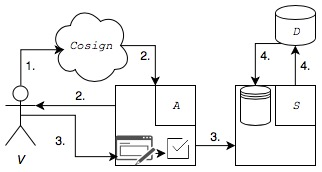
\includegraphics[scale=0.9]{images/Voting1}
\caption{Voting phase of~our scheme}
\end{center}
\end{figure}

\subsection{Counting}
\begin{enumerate}
\item Server $S$ is disconnected from~network and off-line mode is enabled.
\item Using a~secured USB device, the~election commission $B$ transfers encrypted votes from~$S$'s internal database of~votes to~machine for~vote counting $M$. It is crucial that \emph{UK logins} stored in~this database be excluded from~the~transfer.
\item With~aid of~at least $k$ members of~election commission $B$, secret key $SK$ is reconstructed. Then, it is inserted into~$M$ and used to~decrypt votes.
\item Decrypted votes are, then, validated by~$M$. All votes that are in~the~right format and follow the~rules of~the~elections are counted and the~final result is published.
\end{enumerate}

\begin{figure}
\begin{center}
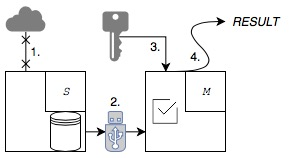
\includegraphics[scale=0.9]{images/Counting1}
\caption{Counting phase of~our scheme}
\end{center}
\end{figure}

\section{Format of~the~Vote}
\label{sek:format}
Definition of~format to~which each vote is formatted prior to~being sent to~the~server for~vote collection $S$ is also part of~our voting scheme. We want the~vote to~be stored in~one compact file and the~choices to~be clearly separated. It is known how many candidates are in~the~elections. Let $M$ be the~number of~candidates. Hence, we propose that the~vote is of~the~following format:
\begin{center}
\texttt{<candidate\_number\_1\#value\_1>...<candidate\_number\_M\#value\_M>}
\end{center}
Here, \texttt{M} is the~representation of~number of~candidates $M$.

This format represents a~string of~ordered pairs $(c_i, v_i)$, where $c_i \in~\{1,...,M\}$ is \newline \texttt{candidate\_number\_i} and $v_i \in~O$ is \texttt{value\_i}, $i\in~1,...,M$. Value $v_i$ is numerical representation of~one of~the~voting options and $O$ is the~set of~all possible numerical representations. For~example, 1 represents YES, 0 represents NO and $O = \{0, 1\}$. 

Let $(c_1, ..., c_M)$ be an~ordered set of~all candidate numbers. Then, $(c_1, ..., c_M)$ is a~permutation of~$\{1,...,M\}$.

It is obvious that the~candidate number 1, for~instance, is given YES if and only if the~vote contains exactly one ordered pair of~value $(1, 1)$.

\section{Security Tools Used in~Our Voting Scheme}
\label{sek:cryptography}
In~our voting scheme, we use these cryptographic protocols and schemes as well as security services to~securely transfer and store the~data.
\subsection{S/MIME}
Developed to~provide a~secure way to~send and receive MIME data, S/MIME (Secure/Multipurpose Internet Mail Extensions) consists of~several cryptographic services, such as authentication or data~encryption. Not only can~it be used by~traditional email clients but also by~message transfer services that use cryptographic solutions to~prevent any person from~illegal intervention. In~order to~use any of~the~services provided by~S/MIME, one must obtain~a~certificate from~a~certificate authority, which they then must install. S/MIME uses asymmetric cryptography based on \emph{PKCS\#7} standard.

%We use only data~encryption provided by~S/MIME. Therefore, we focus on describing this cryptographic service.

Ramsdell and Turner provide a~detailed specification of~S/MIME Version 3.2 in~\cite{Ramsdell}. More can~be also read in \cite{Turner} and \cite{SMIME}.
\subsection{Shamir's Secret-Sharing Scheme}
In~\cite{Shamir}, Adi Shamir proposes a~solution to~the~problem of~dividing data~into~$n$ pieces in~such a~way that these data~can~be reconstructed using $k$ of~these $n$ pieces, but attempt to~reconstruct the~data~with~fewer than~$k$ pieces results in~no information about it. Such a~scheme is called \emph{($n,k$)-threshold scheme}. The~scheme he proposed is based on polynomial interpolation. 

Let $p(x)$ be a~polynomial of~degree $d$. It is obvious that $d+1$ distinct points $(x_0, p(x_0)),...,(x_d, p(x_d))$ are sufficient to~define $p(x)$ and that $p(x)$ cannot be defined with~fewer than~$d+1$ distinct points. 
\bigbreak
In~Shamir's scheme, assume that data~$D$ is a~number. Then, to~divide $D$ into~$n$ pieces in~such a~way that it can~be reconstructed by~using at least $k$ pieces, we follow these steps:
\begin{enumerate}
\item We pick a~random $k-1$ degree polynomial $p(x) = a_0 + a_1x + ... + a_{k-1}x^{k_1}$, where $a_0 = D$. 
\item We, subsequently, evaluate $D_1 = p(1), ..., D_n = p(n)$. Then, each of~$n$ distinct pieces of~secret consists of~an~ordered pair $P_i = (i, D_i)$, where $i \in~1...n$.
\item In~order to~reconstruct data, at least $k$ pieces of~secret $P_{i_1}, ... , P_{i_k}$ are put together. Polynomial interpolation is then used to~find $p(x)$, which is the~Lagrange polynomial for~the~set of~used pieces of~secret. This makes recovering data~$D$ possible because $p(0) = a_0$ and $p(x)$ has been constructed in~such a~way that $a_0 = D$.
\end{enumerate}
The~scheme as described above consists only of~the~basic idea~on which secret sharing is based. In~reality, we use modular arithmetic instead of~its real counterpart. Let $p > \max(D, n)$ be a~prime number. Then, the~set of~integer coefficients $a_0, ..., a_{k-1}$ is picked randomly from~a~uniform distribution over integers in~$[0, p)$. Values $D_0, ..., D_n$ are also computed modulo $p$. The~set of~coefficients forms a~field $\mathbb{Z}_p$, which makes polynomial interpolation and data~retrieval possible \cite{Shamir}.

This scheme has some useful properties. It can~be observed that the~individual pieces are at most of the~same size as the~original data. With~$k$ fixed,  some pieces can~be added or deleted without affecting the~other, or the~pieces can~be changes without changing the~original data. It is also possible to~reflect hierarchy in a~particular group, such as election commission, in a~way of distributing the~pieces. For~example, chairperson of the~commission is given three pieces, vice-chairperson two and the~other members one.
%By~solving a~system of~$k$ linear equations,  
\subsection{Cosign}
Comenius University in~Bratislava~uses \emph{Cosign}, a~secure single sign-on web authentication system originally developed at the~University of~Michigan~\cite{Cosign}. It is based on~web cookies. 

Authentication data~are sent to~the~central server, which uses an~authentication protocol to~verify these data. The~server, then, sets the~user a~web cookie, controlled by~\emph{Apache} filters during every user's attempt to~access addresses secured by~the~system. During the~whole process, \emph{TLS} is used for~a~secured communication.

In~chapter \ref{kap:implementation} is described how authentication via~\emph{Cosign} has been integrated into~our system.
%\section{Accomplishment}
%In~this section, we discuss how our solution meets requirements.

\section{Other Proposed Solutions}
In~the~course of~designing the~final voting scheme for~our election system, we proposed some other solutions. Those were either rejected, or the~final scheme was based on them and their modifications.
There are two elementary design classes being in~consideration during the~whole process. Those are based on question whether server gives client any additional information used to~authorise the~sender of~the~vote. Regarding this, we consider two meaningful classes, which we call \emph{authorisation by~a~token} and \emph{authorisation~by~user information}. In~all of~the~schemes we have looked at, at~least three players represented by~computers are needed: a~\emph{client $C$}, an~\emph{authentication server $A$} and a~\emph{counting machine $B$}.

\subsection{Authorisation by~a~token}
In~this design, authorisation in~provided~by~a~\emph{token}. This token assures $B$ that the~vote comes from~an~authorised voter without~associating it with~a~particular voter. In~order to~preserve anonymity, token must be generated or handled with~in~a~way that it cannot be associated with~any particular voter. In~chapter \ref{kap:existing}, we describe some existing solutions using this design. 

Here, we briefly describe voting phase of~a~scheme that uses server $A$'s signature to~prove that the~vote comes from~an~authorised voter. 
\bigbreak
Let $V$ be voter and $n \in~\mathbb{N}$, $n \ge 2$, be constant defined by~the~scheme. Then, for~each voter $V$:
\begin{enumerate}
\item Voter $V$ logs~in~and voting application is opened on $C$.
\item Client $C$ sends $n$ encrypted votes and $V$'s identity to~$A$, where 1 of~those is the~real vote and the~other votes are fake.
\item If $V$ is an~authorised voter, $A$ signs all $n$ votes and sends them back to~$C$.
\item Client $C$ sends the~signed real vote to~$B$.
\item Server $B$ validates the~vote and if it recognises the~signature with~which the~vote is signed, then it stores the~vote.
\end{enumerate}

The~main~issue with~this scheme is that it may enable the~voter to~double-vote when their voting application is corrupted. In~chapter \ref{kap:existing} we introduce the~reader to~David Chaum's scheme, which was designed to~be used with~electronic cash to~prevent double-spending. When using a~modification of~this scheme to~prevent double-voting, we face a~problem. In~order to~achieve this, additional data~about the~voter have to~be generated and stored on client's side. Of~course, these data~cannot be stored on voter's personal computer or smartphone, since our scheme is supposed to~be mobile and these data~have to~be accessed from~any device of~those kinds. This means that a~cloud storage in~which these data~can~be stored has to~be provided. This storage has to~be secured in~a~way that only voter can~freely access the~data. It raises new security tasks, which we think the~reader can~imagine. We do not say that it is impossible to~implement such a~system, but we think that it is not necessary to~implement such a~complex system for~purposes of~our type of~elections.

We have also come up with~a~totally different scheme using mix networks, referred to~in~chapter \ref{kap:existing}, to~mix the~tokens in~order to~assure anonymity.

\begin{figure}[h]
\begin{center}
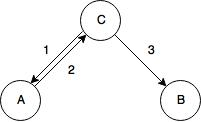
\includegraphics{images/PE2}
\caption{Authorisation by~a~token}
\end{center}
\end{figure}

\subsection{Authorisation by~user information}
Using voting schemes in~this class, $C$ assures that the~vote comes from~an~authorised voter by~providing a~publicly inaccessible piece of~information unique for~that voter that can~be matched with~a~record in~$A$'s memory. In~order to~retain~anonymity, the~vote must be in~an~illegible form during the~whole time it can~be associated with~this piece of~information.

Here, we provide a~simple scheme that has been modified and partly used in~the~final voting scheme.
\bigbreak
Let $V$ be voter. Then, for~each voter $V$:
\begin{enumerate}
\item Voter $V$ logs in~and the~voting application is opened on $C$.
\item Client $C$ sends encrypted vote and $V$'s identity to~$A$.
\item If $V$ is authorised to~vote, then $A$ sends the~encrypted vote without $V$'s identity to~$B$.
\item Server $B$ stores the~vote. 
\end{enumerate}
This scheme has several security issues. Let corrupted $A$ send $B$ encrypted votes and voters' identities. These votes can~be, then, decrypted by~$B$, which also knows who casted which vote. Thus, it can~be revealed how voters voted.
\begin{figure}[h]
\begin{center}
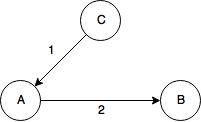
\includegraphics{images/PE1}
\caption{Authorisation by~user information}
\end{center}
\end{figure}










